\documentclass{article}
\usepackage[utf8]{inputenc}
\usepackage{graphicx}
\usepackage{amsmath}

\title{Diffusion}
\date{\today}

\begin{document}
\maketitle
\section{Introduction}
\quad In this problem we aim to simulate the diffusion of one substance diffusion in another(sugar in water for instance). Diffusion will start from a box profile with a peak at origin and 10 grid around and diffuse in 1 dimension. We will found out the diffusion will approximate Gaussian distribution at later times and fit will be preformed to verify that $\sigma=\sqrt{2Dt}$ for several snapshot t.

\section{Part a}
\quad First of all we will show analytically that the spatial expectation $\langle x(t)^2\rangle$ of the 1D normal distribution $\rho_{(x,t)}=\frac{1}{\sqrt{2\pi}\sigma{(t)}}exp(-\frac{x^2}{2\sigma{(t)}^2})$ is just $\sigma(t)^2$.

The spatial expectation
\begin{equation}
\begin{split}
\langle x(t)^2\rangle&=\int_{-\infty}^{\infty}\frac{1}{\sqrt{2\pi}\sigma(t)}x^2exp(-\frac{x^2}{2\sigma(t)^2})dx\\
&=\sigma(t)^2.
\end{split}
\end{equation}

So $\langle x(t)^2\rangle=\sigma(t)^2$
\section{Part b}
\quad We know the diffusion equation
\begin{equation}
\frac{\partial\rho}{\partial t}=D\nabla^2\rho
\end{equation}
If we discretize time and position to $t=k\Delta t, x=i\Delta x$, we can get the recursion equation with time, 
\begin{equation}
\rho_{i,k+1}=\rho_{i,k}+D\frac{\Delta t}{\Delta x^2}(\rho_{i+1,k}+\rho_{i-1,k}-2\rho_{i,k})
\end{equation}
here we used $\Delta t=0.002s, \Delta x=0.1m, D=2$. The relation $\Delta t=\frac{\Delta x^2}{2D}$ is satisfied to guarantee convergence.

Then, with the initial distribution given, all future state can be solved. We here will solve the equation for 150s and take snapshot at 30s, 60s, 90s, 120s and 150s. Gaussian fit is applied to these snapshot to verify $\sigma=\sqrt{2Dt}$. Plots for the 5 snapshots and fitted Gaussian are shown in Figure 1.
\begin{figure}
\centering
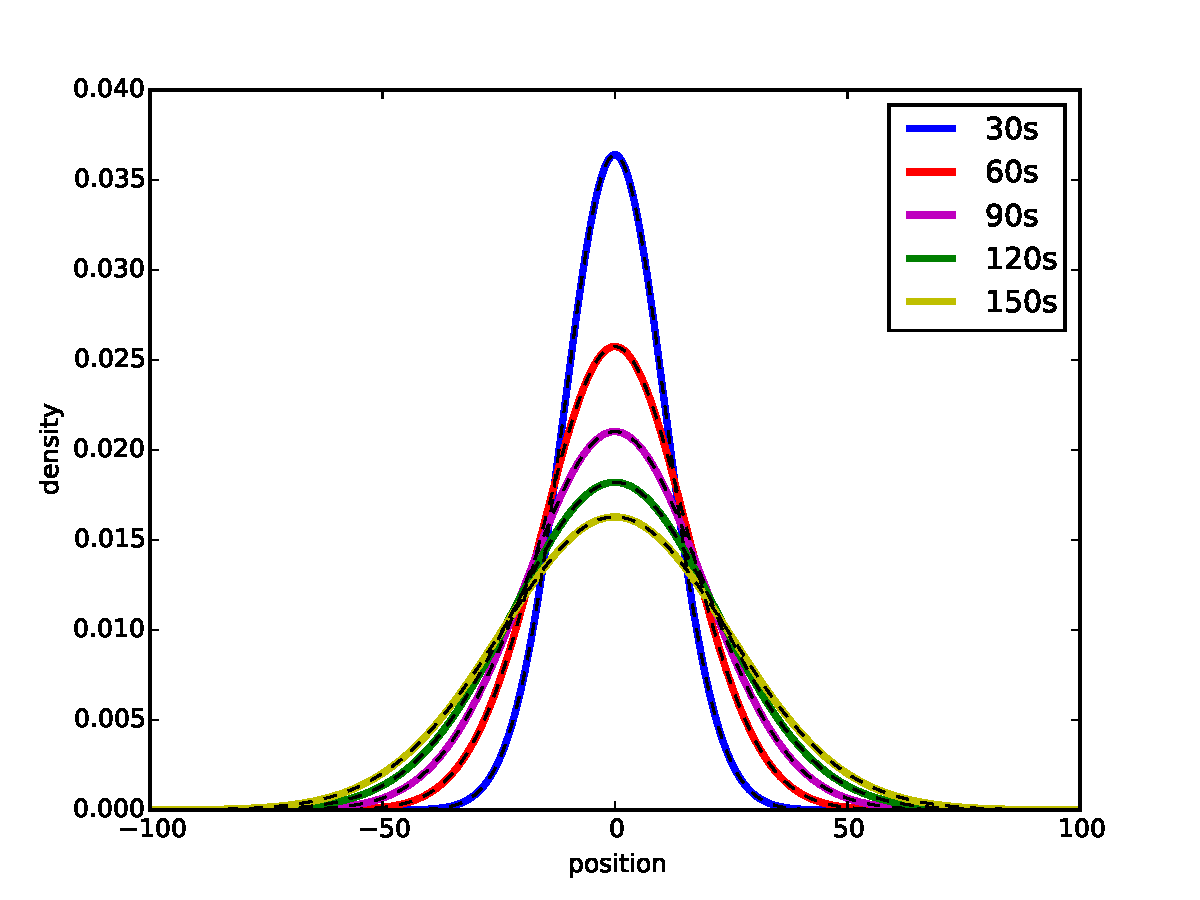
\includegraphics[scale=0.85]{diffusion.pdf}
\caption{Snapshots at 30s, 60s, 90s, 120s, 150s and comparison with fitted curve}
\end{figure}

As for the Gaussian fit, we used the function curve\_fit from scipy.optimize. We first define the Gaussian function with input of $x, \mu, \sigma$ and call it in the function \_fit to get the optimized $\sigma$ the comparison of $\sigma$ with $\sqrt{2Dt}$ are shown in Figure 2.
\begin{figure}
\centering
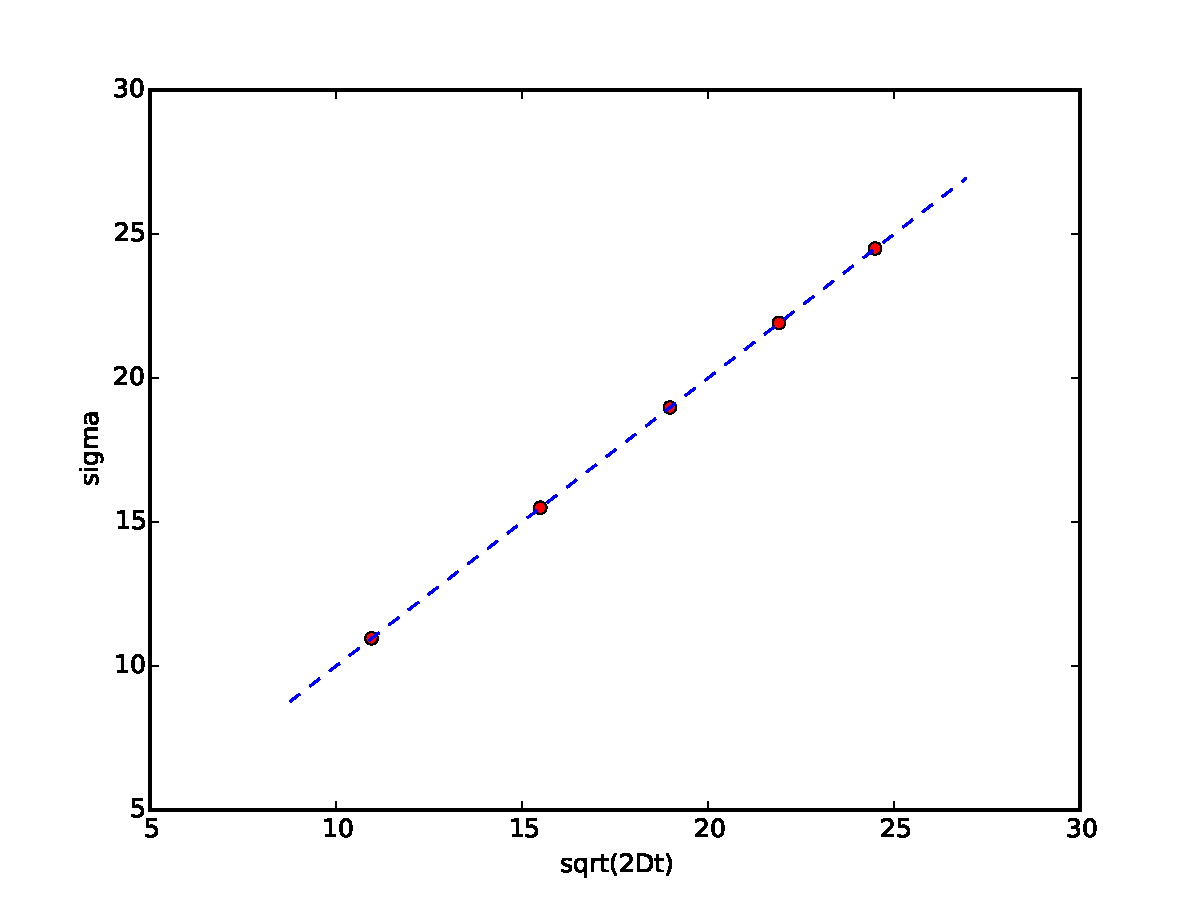
\includegraphics[scale=0.75]{sigma.pdf}
\caption{Comparison of $\sigma$ and $\sqrt{2Dt}$, the blue dashed line is y=x.}
\end{figure}

\section{Discussion}
\quad In this problem, we used the diffusion equation to simulate the diffusion of a initial distribution of a peak(spread out a few grid) and we find that the distribution tend to approximate Gaussian distribution. We also find that the spatial spread expectation $\langle x(t)^2\rangle=2Dt$ increase linearly with time.






\end{document}
